\subsection{Backward Stepwise Selection}

The second method applied is the dual of the previous one, i.e.\ \textit{Backward Stepwise Selection}. The model obtained is shown in \Fig~\ref{fig:BackwardModelSummary}.
\begin{figure}[h]
	\centering
	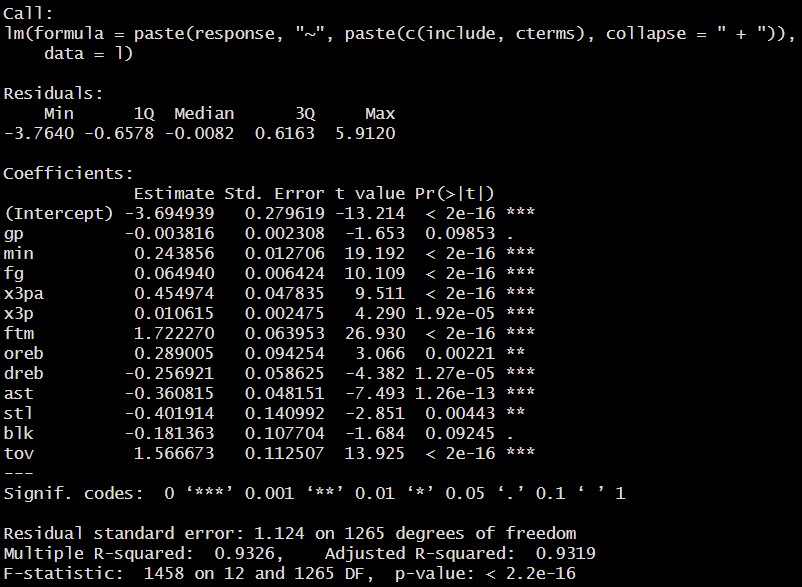
\includegraphics[width=0.35\linewidth]{ImageFiles/Regression/Backward/BackwardModelSummary}
	\caption{Backward Stepwise Selection Output Model.}
	\label{fig:BackwardModelSummary}
\end{figure}

The model obtained with this algorithm includes 12 variables, one less than Forward Stepwise. Upon comparing the two models, we found that they have the same variables, with the exception of \textit{"X3P\_MADE"}, that was included additionally in the Forward Stepwise model, despite not being significant.
Therefore all the considerations made previously still hold.

However, after removing the non significant variables the obtained models by the two algorithms are the same, suggesting that the selection is good.